\section{Accelerometer}

MotionSensor giver adgang til accelerometret der angiver accelerationen i x,y,z retningerne.

\subsection{Gangart}
Vi forestiller os at man kan analysere på patientens gangart for at se om patienten går i et normalt tempo eller om patienten slæber hen ad gulvet.
For at finde dette er det muligvis nødvendigt at benytte gyro sensoren sammen med accelerometret.
Endvidere kan det være at man skal vide hvilken retning tyngdekræften trækker.

\subsection{Aktivitetsniveau}
Baseret på det vi har hørt fra Morten, er motion og aktivitet vigtigt for personer med psykiske sygdomme og hvis de ikke rører på sig særlig meget kan det være en indikator for hvilken slags sinds situation de befinder sig i.
For at estimere patientens aktivitetsniveau kan accelerometret bruges, da vi baseret på den kan se om de bevæger telefonen. 

\subsection{Nattesøvn}
Accelerometret kan også benyttes til at overvåge patientens nattesøvn og derved undersøge om den er rolig eller meget forstyrret.


\subsection{Visualisering} Normal 2 dimensionel graf som viser aktivitets niveau over flere dage, uger, måneder. Muligivis en kalender der hvis hvor aktiv man har været på en bestemt dato, så en dato man har været meget aktiv er grøn, og en dato hvor man har været meget lidt aktiv er datoen rød.

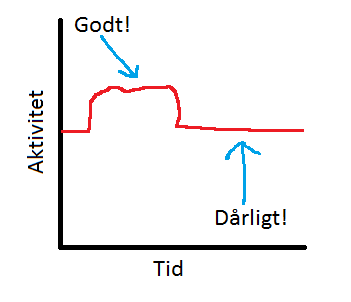
\includegraphics{graphics/aktivitet_billed}

\subsection{Kort oprids af fremgangsmåde} Hvis det skal bruges til at tracke hvordan en person bevæger sig, kan man bruge et bayesiansk netværk der benytter sig af de fysiskelove, hvor gyroskopet kan være meget behjælpelig. Ved rystelser, kan man se på hvor meget personer ryster i dagligdagen, og derefter se om personen ryster mere på nogle bestemte tidspunkter. For aktivitetsniveau kan man på hvor meget og ofte at man accelerer/deaccelerer, og udfra dette bedømme om man dyrker noget aktivt.